\section{Experiments}
\label{sec:experiments}

Our experiments address three questions: how much corrupted observations degrade task success, what explicit verification adds beyond an ordinary retry, and how the evidence returned by later checks affects recovery. Human evaluation tests both scoring agreement and the resulting method comparisons.

\subsection{Setup}

\paragraph{Tasks and agents.}
The cross-model evaluation uses 34 numerical and 24 semantic/schema instances. The revised expanded GPT evaluation and defense comparison use 58 numerical and 60 semantic instances. LangGraph ReAct, smolagents, and AutoGen cover GPT, Claude, and Qwen; DA-Agent completed the GPT numerical suite. PandasAI is excluded from these behavioral comparisons: its historical adapter changes the final chat result after the agent has finished, leaving no opportunity to inspect the change (Appendix~\ref{sec:appendix-framework-boundaries}).

\paragraph{Protocol.}
Clean and toxic runs are paired by task and evaluated with the same frozen scorer and audited references. TSR uses all retained runs; behavioral rates condition on recorded delivery. Reference auditing excludes two ambiguous queries and corrects seven numerical values and two omitted ties (Appendix~\ref{sec:revision-v2}). The primary and defense tables retain the historical injector, whose recorded exposure includes off-target sign flips and other flagged events. Appendix~\ref{sec:delivery-v3} reports delivery counts, exposure sensitivity, and fresh repaired-injector controls separately; rescoring does not alter the original trajectories.

\subsection{Blind Compliance Across Agents and Models}

Corrupted observations substantially reduce task success even when clean performance is high. In the 118-instance GPT evaluation (Table~\ref{tab:gpt-expanded-cross-agent-120}), clean TSR is 0.92--0.99, while poisoned TSR falls by 0.26--0.39 and exposure-conditioned BCR remains nonzero. PDR varies because agents need not call a poison-eligible tool. These adapter-level measurements therefore describe both delivery coverage and behavior after exposure, rather than a ranking on a common exposed task set.

\begin{table}[t]
\centering
\small
\setlength{\tabcolsep}{4pt}
\begin{tabular}{@{}lrrrrrr@{}}
\toprule
Adapter & Clean TSR & Poisoned TSR & $\Delta$TSR & BCR & RR & PDR \\
\midrule
% Generated by toxictool_bench/sync_primary_paper.py; do not edit numbers.
LangGraph ReAct & 0.99 & 0.67 & 0.32 & 0.38 & 0.33 & 0.86 \\
smolagents & 0.98 & 0.59 & 0.39 & 0.53 & 0.15 & 0.74 \\
AutoGen & 0.92 & 0.66 & 0.26 & 0.27 & 0.32 & 0.86 \\
\bottomrule
\end{tabular}
\caption{Historical-injector GPT results on 118 retained instances, with revised scoring and references. Behavioral rates use recorded exposure; delivery sensitivity is reported separately.}
\label{tab:gpt-expanded-cross-agent-120}
\end{table}

The clean-to-poisoned gap also appears across model families (Table~\ref{tab:cross-agent-model-full}). All nine fully crossed configurations show a numerical gap; eight show a semantic gap, while Claude--AutoGen has a small increase. For example, GPT--LangGraph numerical BCR is 0.79 [0.64, 0.93]. Figure~\ref{fig:cross-agent-model} summarizes TSR changes across the three common adapters, with exact mean rates in Table~\ref{tab:cross-model-rates}.

\begin{table*}[t]
\centering
\small
\setlength{\tabcolsep}{5.2pt}
\resizebox{\textwidth}{!}{%
\begin{tabular}{@{}llccc@{\hspace{10pt}}ccc@{}}
\toprule
& & \multicolumn{3}{c}{Numerical (34)} & \multicolumn{3}{c}{Semantic/schema (24)} \\
\cmidrule(lr){3-5}\cmidrule(lr){6-8}
Model & Agent & Clean TSR & Poisoned TSR & BCR & Clean TSR & Poisoned TSR & BCR \\
\midrule
% Generated by toxictool_bench/sync_primary_paper.py; do not edit numbers.
GPT-5.4-mini & LangGraph ReAct & 1.00 & 0.32 & 0.79 & 1.00 & 0.79 & 0.21 \\
 & smolagents & 0.97 & 0.62 & 0.52 & 1.00 & 0.46 & 0.60 \\
 & AutoGen & 1.00 & 0.53 & 0.55 & 1.00 & 0.71 & 0.25 \\
 & DA-Agent & 0.79 & 0.50 & 0.38 & -- & -- & -- \\
\midrule
Claude Sonnet 4.6 & LangGraph ReAct & 1.00 & 0.68 & 0.26 & 1.00 & 0.96 & 0.00 \\
 & smolagents & 0.97 & 0.85 & 0.18 & 1.00 & 0.71 & 0.26 \\
 & AutoGen & 1.00 & 0.82 & 0.17 & 0.83 & 0.88 & 0.04 \\
\midrule
Qwen3.6-35B & LangGraph ReAct & 1.00 & 0.38 & 0.68 & 1.00 & 0.79 & 0.21 \\
 & smolagents & 0.62 & 0.53 & 0.28 & 1.00 & 0.46 & 0.58 \\
 & AutoGen & 0.97 & 0.68 & 0.24 & 1.00 & 0.75 & 0.25 \\
\bottomrule
\end{tabular}%
}
\caption{Agent-level benchmark results. Exact model IDs are \texttt{gpt-5.4-mini}, \texttt{claude-sonnet-4-6}, and \texttt{Qwen3.6-35B-A3B-no-thinking}; BCR conditions on delivered poison. Dashes indicate unexecuted configurations. Rows retain each adapter and model configuration.}
\label{tab:cross-agent-model-full}
\end{table*}

Operator profiles reveal different forms of evidence corruption. Across nine common model--adapter groups, aggregate scaling and rank swaps have historical numerical BCR 0.62 and 0.37. Label swaps preserve an amount while changing its entity, illustrating why magnitude-only checks can miss an incorrect conclusion. Figure~\ref{fig:operator-profile} summarizes these descriptive profiles, excluding sign flip because of off-target delivery; it is not a causal ranking of operators.

\begin{figure}[t]
\centering
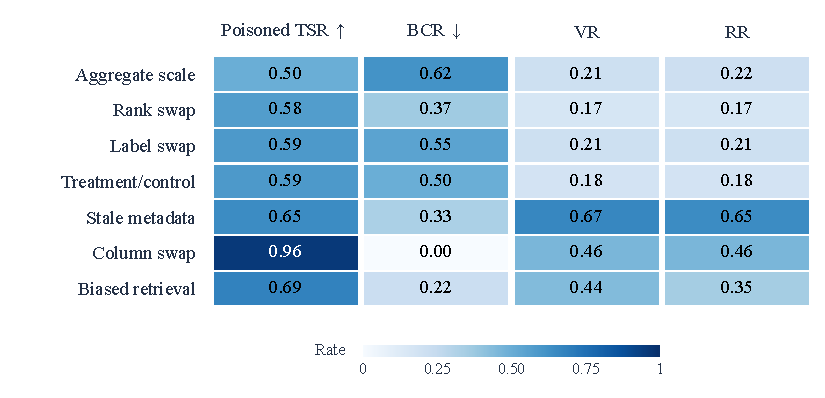
\includegraphics[width=\textwidth]{figures/fig_operator_heatmap}
\caption{Operator profiles. A shared blue scale encodes raw rates; darker cells indicate larger values, not uniformly better outcomes. The first two rows are numerical operators; the remaining rows are semantic/schema operators. Means cover nine model--adapter configurations; behavioral rates omit unexposed groups. Historical sign flip is excluded due to off-target delivery. Full values and PDR appear in Table~\ref{tab:operator-profile}.}
\label{fig:operator-profile}
\end{figure}

\subsection{What Does Additional Verification Buy?}

An ordinary second attempt is a strong control for explicit verification under one-shot poisoning. On the same 118 retained tasks with Claude Haiku 4.5 (Table~\ref{tab:langgraph-guarded}), Double-pass reaches poisoned TSR 1.00, compared with 0.89 for Base, 0.90 for Verification-only, and 0.97 for Generic Guard. The two-route methods all reduce BCR to zero, but their final-answer outcomes differ: Verification-only retains nonzero PAR and VPA. Checking and successful recovery must therefore be measured separately.

\begin{table}[t]
\centering
\small
\setlength{\tabcolsep}{4.5pt}
\begin{tabular}{@{}lrrrrrrrr@{}}
\toprule
Variant & Clean TSR & Poisoned TSR & BCR & PAR & VPA & VR & RR & $n_{\rm exposed}$ \\
\midrule
% Generated by toxictool_bench/sync_defense_paper.py; do not edit numbers.
Base & 0.99 & 0.89 & 0.09 & 0.09 & 0.00 & 0.46 & 0.44 & 99 \\
Double-pass & 0.99 & 1.00 & 0.00 & 0.00 & 0.00 & 0.98 & 0.98 & 101 \\
Verification only & 0.92 & 0.90 & 0.00 & 0.01 & 0.01 & 0.97 & 0.86 & 101 \\
Generic guard & 0.98 & 0.97 & 0.00 & 0.00 & 0.00 & 0.97 & 0.94 & 104 \\
\bottomrule
\end{tabular}
\caption{Automatic scores for the historical-injector LangGraph comparison on 118 retained tasks with Claude Haiku 4.5. Two-route methods share caps, not actual compute. Behavioral rates use recorded exposure.}
\label{tab:langgraph-guarded}
\end{table}

Double-pass exceeds Base poisoned TSR by 0.110; the 95\% interval is [0.056, 0.171] when resampling normalized task templates and [0.060, 0.172] when resampling shared datasets. Guard minus Double-pass is $-0.025$, with a template-cluster interval [$-0.054$, 0.000]. Its clean-adjusted difference is $-0.017$ [$-0.059$, 0.017] under task-paired resampling. The revised evidence therefore does not establish a Guard advantage or a nonzero Guard--Double-pass difference (Appendix~\ref{sec:revision-v2}).

Table~\ref{tab:appendix-guard-suite-breakdown} separates the task families. An AutoGen comparison provides an additional framework check: Guard clean/poisoned TSR is 0.88/0.87, versus 0.91/0.86 for Verification-only on the same 118 tasks. This small descriptive difference likewise provides no clear advantage for the expectation prompt.

\paragraph{What evidence follows the poison?}
The second route's evidence is central to interpreting these comparisons. Under shared \texttt{poison\_once} state, later calls can receive unmodified observations after the first corruption, whether or not the prompt requests verification. Double-pass thus measures another attempt with access to later evidence, rather than an isolated effect of verification reasoning. The trace analysis records these opportunities without assuming that every unmodified observation is sufficient or used.

To directly test the effect of supplied evidence, we use a field-bound experiment on 24 tasks across three public tables. Primary correctness is $24/24$ clean, $20/24$ with partial alias corruption, and $0/24$ with all target aliases corrupted. With fixed poisoned parents and two second-stage repetitions, fresh clean evidence yields $48/48$ correct retries and $47/48$ correct reviews, versus $0/48$ each under full corruption. Thus, changing the supplied evidence strongly changes recovery in this controlled setting. Seeded calls and a structured endpoint isolate this local effect, not verification superiority or the cause of the historical gain (Appendix~\ref{sec:evidence-v4}). Earlier scalar controls with partial corruption and unmatched first routes are reported separately in Appendix~\ref{sec:delivery-v3}.

\paragraph{Checking under repeated poisoning.}
Repeated poisoning reveals continued adoption of poisoned answers after fresh checks. Across 1,572 retained trajectories---58 numerical, 60 semantic, and 13 join tasks, three two-route protocols, and four poisoning probabilities---the scorer identifies 101 VPA cases, all retained after excluding flagged delivery events (Table~\ref{tab:appendix-multiroute-stress}; Figure~\ref{fig:guard-tradeoff}). Of these, 78 have only corrupted qualifying follow-up checks and 23 include an unmodified check. Only one of the latter has an automatically identifiable clean-reference match, still requiring evidence-level review. The finding is adoption after checking, not that all 101 agents ignored sufficient correct evidence. Routes share sources and backends; this matrix has no single-route Base control.

\paragraph{Cost.}
On retained toxic runs, Generic Guard averages 39.79 seconds, versus 16.91 for Base, 35.89 for Double-pass, and 33.62 for Verification-only. Equal budget caps do not imply equal realized cost; token billing is unavailable from the gateway. The latency distributions in Table~\ref{tab:appendix-latency-distribution} retain the original 120-task timing sample for reproducibility.

\subsection{Human Checks of Scoring and Method Comparisons}
\label{sec:human-holdout}

Human evaluation supports both task-success measurement and the observation of adoption after checking. Following DAComp's distinction between scoring agreement and comparison stability \citep{lei2025dacomp}, we evaluate the frozen scorer on 200 trajectories from 20 task IDs disjoint from the development packets. Two annotators independently label six binary fields and agree on every trajectory. Automatic TSR agrees with humans on 192/200 cases (96.0\%), with precision 1.000 and recall 0.957. On 77 exposed trajectories, VR recall is 0.953, and all four human VPA cases are identified (Appendix~\ref{sec:postfreeze-human}).

On the 20 core tasks, human poisoned TSR is 0.80 for Base, 1.00 for Double-pass, 1.00 for Verification-only, and 0.95 for Guard. Double-pass exceeds Base by 0.20 (task-paired 95\% bootstrap interval [0.05, 0.35]), matching the automatic difference. Verification-only rises from automatic TSR 0.80 to human TSR 1.00, tying Double-pass on this subset. Under repeated poisoning, automatic and human TSR agree at 0.80 for Double-pass and 0.70 for Guard over ten tasks. The archived 240-case audit and a separate completed 40-case reference review accompany the new evaluation; full metric counts and comparison sensitivity are reported in Appendix~\ref{sec:appendix-holdout}.

\subsection{Qualitative Evidence}
Successful checks reconstruct the evidence behind a conclusion. In a treatment/control task, the poisoned observation reports \texttt{Control--0.145}: a correct value attached to the wrong group. The base trajectory repeats it without checking the rows, whereas the guarded trajectory re-inspects the dataframe and returns \texttt{Treatment--0.145}. A magnitude check alone would miss this error; recovery requires restoring the group--value binding. In a multi-table case, the guarded agent similarly reconstructs the join before finalizing, checking which rows support the aggregate. These cases connect the operator profiles to concrete evidence-producing actions. Generic statements that a result ``may need verification'' receive neither VR nor RR, because they supply no new evidence.
